
\begin{titlepage}
    % Strona tytułowa
    %\vbox to\textheight{\hyphenpenalty=10000
    \begin{center}
	\begin{tabular}{p{107mm} p{9cm}}
	    \begin{minipage}{9cm}
	      \begin{center}
	      Politechnika Warszawska \\
	      Wydział Elektroniki i~Technik Informacyjnych \\
	      Instytut Informatyki
	      \end{center}
	    \end{minipage}
	    &
	    \begin{minipage}{8cm}
	    \begin{flushleft}
	     \footnotesize
	      Rok akademicki 2013/2014
	    \vspace*{2.75\baselineskip}
	    \end{flushleft}
	    \end{minipage} \\
	\end{tabular}
	\vspace*{1.75\baselineskip}
	\par\vspace{\smallskipamount}
	\vspace*{2\baselineskip}{\LARGE Praca dyplomowa inżynierska\par}
	\vspace{3\baselineskip}{\LARGE\strut Andrzej Niedźwiedź\par}
	\vspace*{2\baselineskip}{\huge\bfseries System ewidencji zabytków archeologicznych przy użyciu technologii Vaadin\par}

	\vspace*{4\baselineskip}
	\hfill\mbox{}\par\vspace*{\baselineskip}\noindent
	\begin{tabular}[b]{@{}p{3cm}@{\ }l@{}}
	    {\large\hfill } & {\large }
	\end{tabular}
	\hfill
	\begin{tabular}[b]{@{}l@{}}
	Opiekun pracy: \\[\smallskipamount]
	{\large dr inż. Jakub Janusz Koperwas}
	\end{tabular}\par
	\vspace*{4\baselineskip}
    \begin{tabular}{p{\textwidth}}
    \begin{flushleft}
	\begin{minipage}{7cm}
	Ocena \dotfill
	\par\vspace{1.6\baselineskip}
	\dotfill
	\par\noindent
	\centerline{\footnotesize Podpis Przewodniczącego} \par
	\centerline{\footnotesize Komisji Egzaminu Dyplomowego}\par
	\end{minipage}
    \end{flushleft}
    \end{tabular}
    \end{center}}

    % Życiorys
    \newpage\thispagestyle{empty}
    \begin{tabular}{p{5cm} p{12cm}}
    \begin{minipage}{5cm}
    \center
    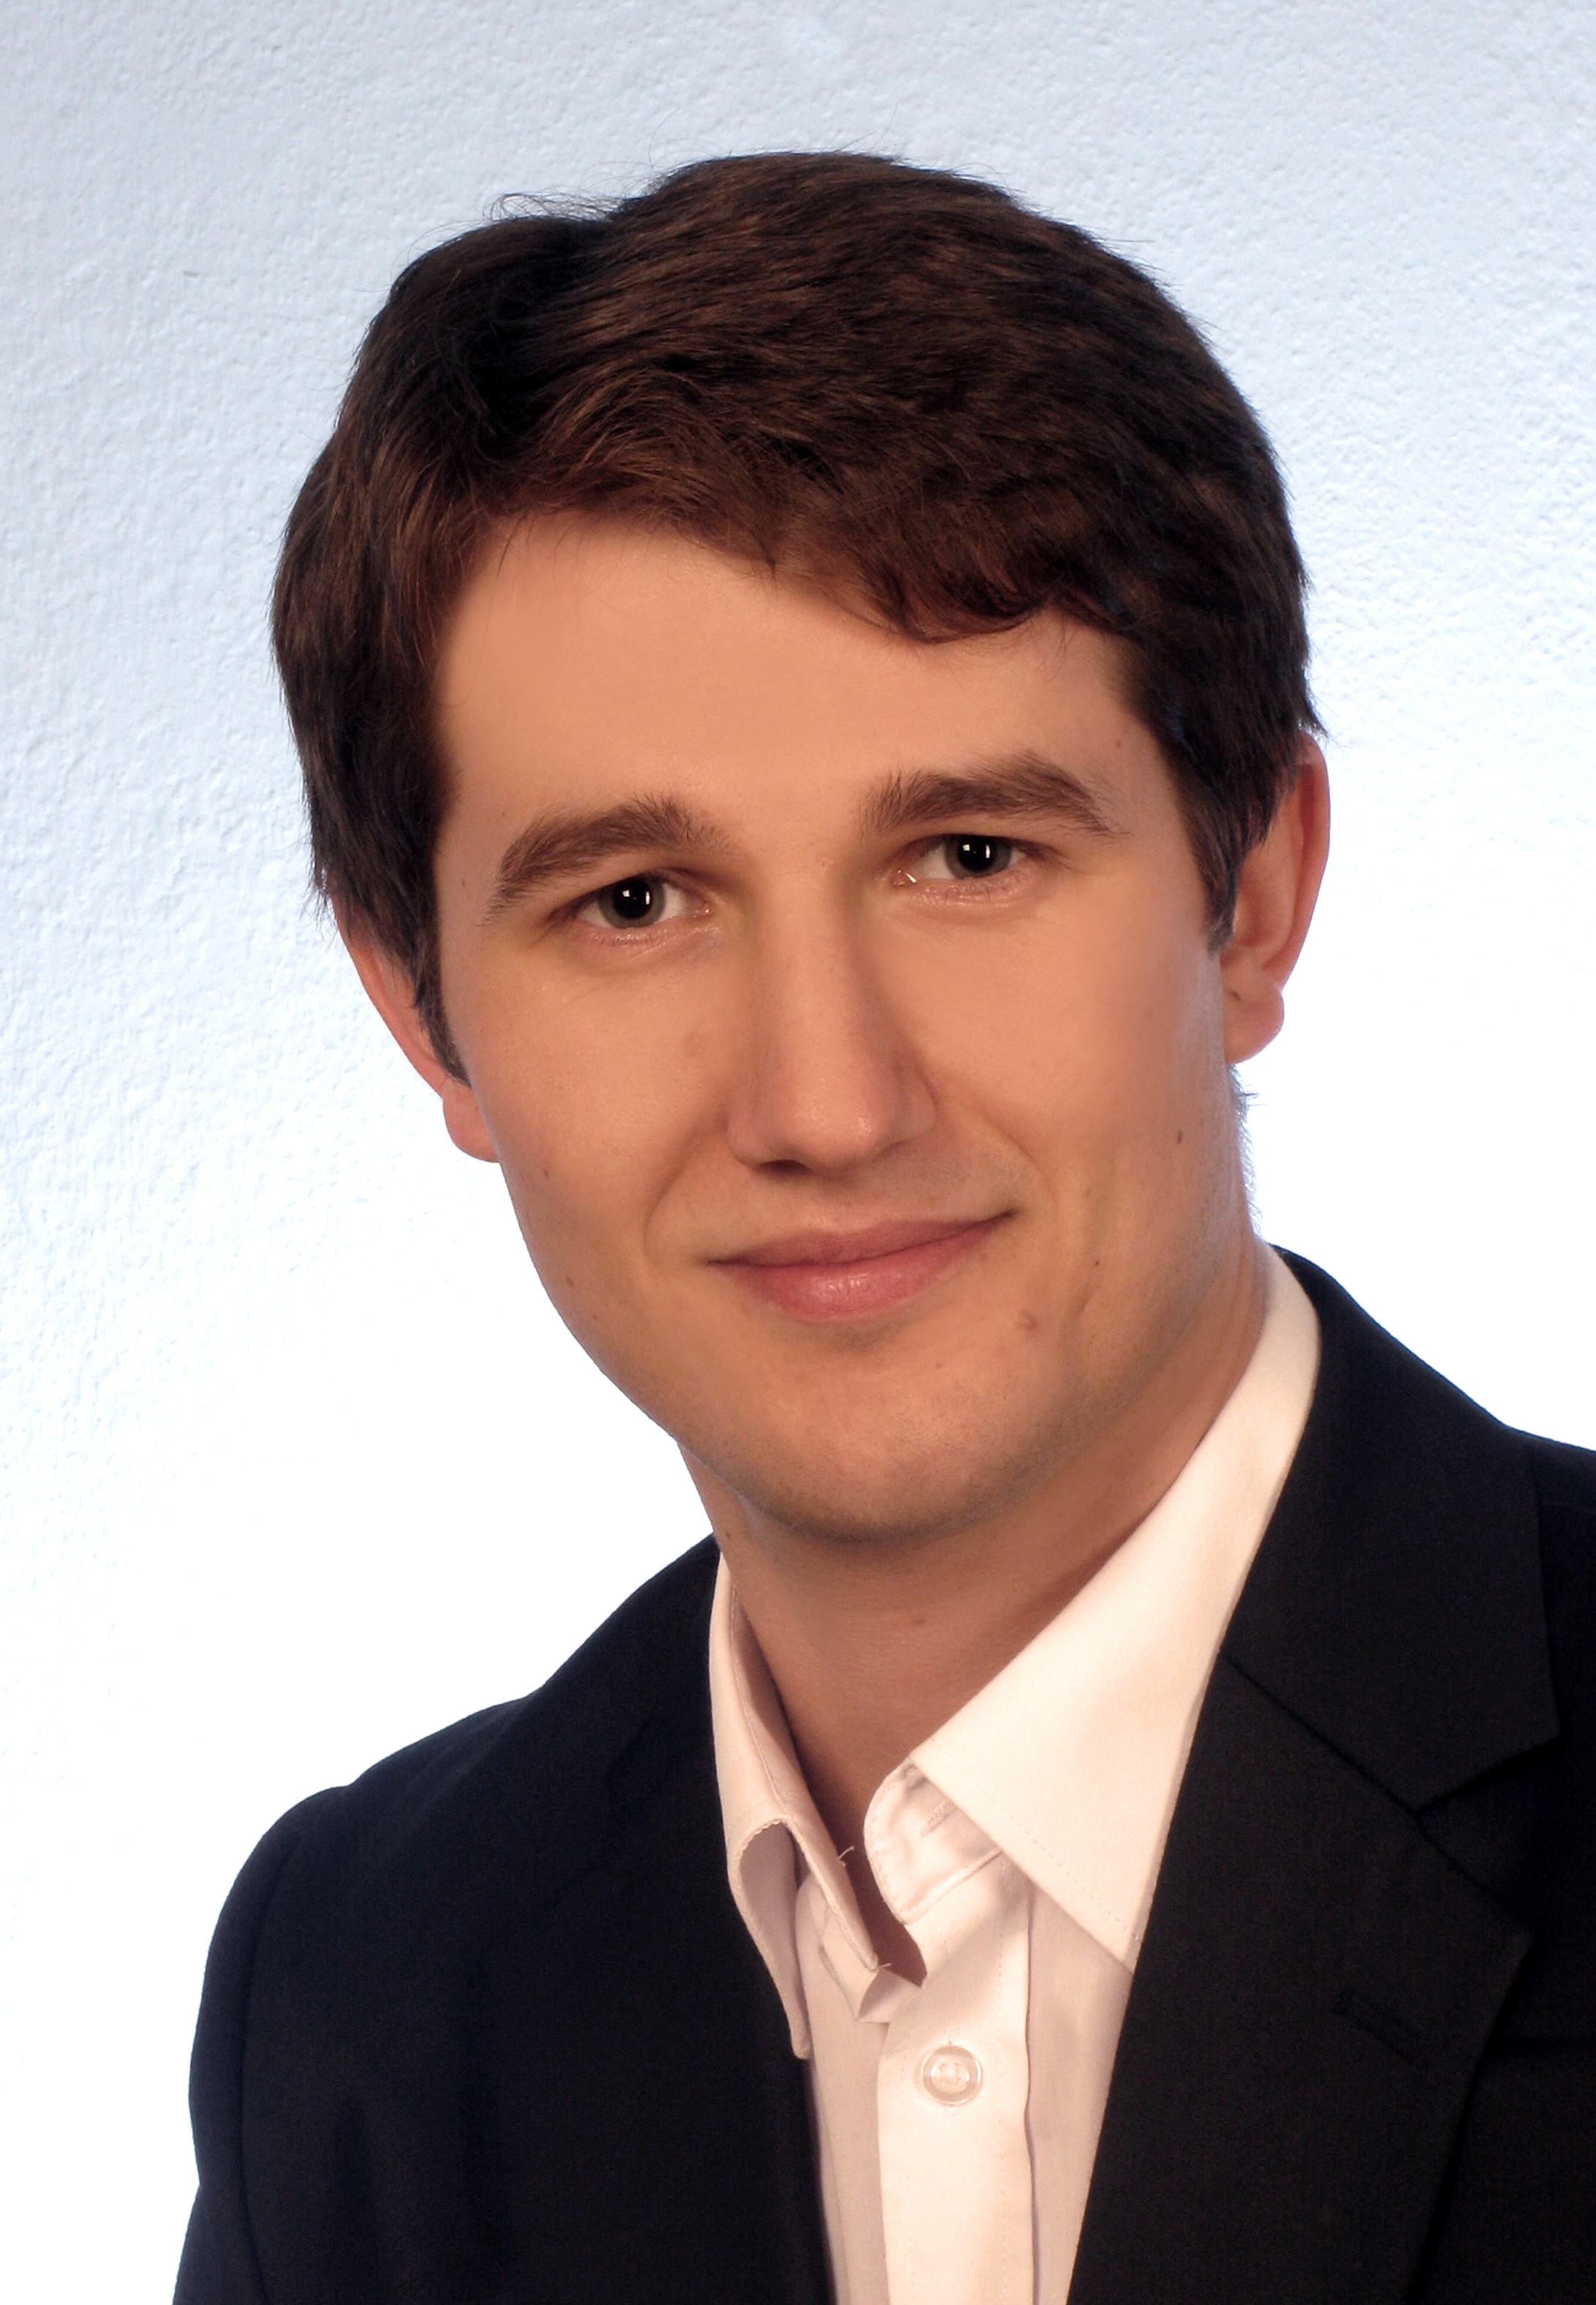
\includegraphics[height=6.5cm,width=4.5cm]{img/foto.jpg}
    \end{minipage}
    &
    \begin{minipage}{12cm}
    \begin{flushleft}
    \par\noindent\vspace{1\baselineskip}
    \begin{tabular}[h]{l l}
	{\normalsize\it Kierunek:} & {\normalsize Informatyka} \\ \\
    {\normalsize\it Specjalność:} & {\normalsize Inżynieria Systemów} \\ & {\normalsize Informatycznych}  \\ \\
    {\normalsize\it Data urodzenia:} & {\normalsize 12 grudnia 1991~r.} \\ \\
    {\normalsize\it Data rozpoczęcia studiów:} & {\normalsize 1 października 2010 r.} \\ \\
    \end{tabular}
    \par\noindent\vspace{1\baselineskip}
    \end{flushleft}
    \end{minipage}
    \end{tabular}
    \vspace*{1\baselineskip}
    \begin{center}
	{\large\bfseries Życiorys}\par\bigskip
    \end{center}

    \indent
    Urodziłem się 12 grudnia 1991 roku w Zamościu. W 2010 roku ukończyłem Społeczne Liceum Ogólnokształcące im. Unii Europejskiej w Zamościu. W październiku 2010 roku rozpocząłem studia na kierunku Informatyka na Wydziale Elektroniki i Technik Informacyjnych na Politechnice Warszawskiej. Od trzeciego roku studiów jestem na specjalizacji Inżynieria Systemów Informatycznych.
    \par
    \vspace{2\baselineskip}
    \hfill\parbox{15em}{{\small\dotfill}\\[-.3ex]
    \centerline{\footnotesize podpis studenta}}\par
    \vspace{1\baselineskip}
    \begin{center}
 	{\large\bfseries Egzamin dyplomowy} \par\bigskip\bigskip
    \end{center}
    \par\noindent\vspace{1.5\baselineskip}
    Złożył egzamin dyplomowy w dn. \dotfill
    \par\noindent\vspace{1.5\baselineskip}
    Z wynikiem \dotfill
    \par\noindent\vspace{1.5\baselineskip}
    Ogólny wynik studiów \dotfill
    \par\noindent\vspace{1.5\baselineskip}
    Dodatkowe wnioski i uwagi Komisji \dotfill
    \par\noindent\vspace{1.5\baselineskip}
    \dotfill

    % Streszczenie
    \newpage\thispagestyle{empty}
    \vspace*{2\baselineskip}
    \begin{center}
	{\large\bfseries Streszczenie}\par\bigskip
    \end{center}

    {\itshape
    Przedmiotem niniejszej pracy jest stworzenie systemu wspierającego ewidencje i tworzenie dokumentacji badań archeologicznych. Aplikacja ta została zaimplementowana z użyciem technologii zaproponowanej przez promotora - szkieletu aplikacji Vaadin - której zbadanie jest równoległym celem. Początek pracy poświęcony jest opisowi zakresu pracy. Następnie przedstawiony został opis systemu oraz wymagania mu stawiane. W dalszej części pracy są wymienione i opisane technologie, które zostały użyte do stworzenia systemu. Dalej przedstawiony jest opis implementacji z naciskiem na architekturę rozwiązania. W kolejnej części znajduje się przedstawienie produktów, które powstały przy okazji tworzenia systemu. Ostatnia część pracy zawiera podsumowanie oraz wnioski płynące z prac nad systemem.}
    \vspace*{1\baselineskip}

    \noindent{\bf Słowa kluczowe}: {\itshape Vaadin, Archeologia, Dokumentacja Archeologiczna}
    \par
    \vspace{4\baselineskip}
    \begin{center}
	{\large\bfseries Abstract}\par\bigskip
    \end{center}
    \noindent{\bf Title}: {\itshape 
	System to support the creation of archeological documentation created using Vaadin framework}\par
    \vspace*{1\baselineskip}
    {\itshape
    This thesis describes web application using three-tier architecture and Java programming language, which purpose was to support making documentation after archaeological research. The following chapters present stages of application preparation. Whole graphic interface was made in framework Vaadin - which is described in detail in one of the chapters}
    \vspace*{1\baselineskip}

    \noindent{\bf Key words}: {\itshape Vaadin, Archeology, Archaeological Documentation}

\end{titlepage}

% ex: set tabstop=4 shiftwidth=4 softtabstop=4 noexpandtab fileformat=unix filetype=tex spelllang=pl,en spell:
